% THIS IS SIGPROC-SP.TEX - VERSION 3.1
% WORKS WITH V3.2SP OF ACM_PROC_ARTICLE-SP.CLS
% APRIL 2009
%
% It is an example file showing how to use the 'acm_proc_article-sp.cls' V3.2SP
% LaTeX2e document class file for Conference Proceedings submissions.
% ----------------------------------------------------------------------------------------------------------------
% This .tex file (and associated .cls V3.2SP) *DOES NOT* produce:
%       1) The Permission Statement
%       2) The Conference (location) Info information
%       3) The Copyright Line with ACM data
%       4) Page numbering
% ---------------------------------------------------------------------------------------------------------------
% It is an example which *does* use the .bib file (from which the .bbl file
% is produced).
% REMEMBER HOWEVER: After having produced the .bbl file,
% and prior to final submission,
% you need to 'insert'  your .bbl file into your source .tex file so as to provide
% ONE 'self-contained' source file.
%
% Questions regarding SIGS should be sent to
% Adrienne Griscti ---> griscti@acm.org
%
% Questions/suggestions regarding the guidelines, .tex and .cls files, etc. to
% Gerald Murray ---> murray@hq.acm.org
%
% For tracking purposes - this is V3.1SP - APRIL 2009

\documentclass{acm_proc_article-sp}
\usepackage[utf8]{inputenc}
\usepackage[T1]{fontenc}
\usepackage{ngerman}
\usepackage{tikz}
\usetikzlibrary{arrows,positioning,fit,shapes,shapes.multipart, calc,shapes.geometric}
\usepackage{varwidth}
\usepackage{listings}
\usepackage{url}

\clubpenalty = 10000
\widowpenalty = 10000

\def\sharedaffiliation{%
\end{tabular}
\begin{tabular}{c}}

\begin{document}

\title{Hybrid or native - what to choose?}

\numberofauthors{6}
\author{
\alignauthor Matthias Altstadt\\
      \email{matthias.altstadt@fau.de}
\alignauthor Tobias Fertig\\
      \email{tobias.fertig@fau.de}
\alignauthor Christian Happ\\
      \email{christian.happ@fau.de}
\and
\alignauthor Daniel Knogl\\
      \email{daniel.knogl@fau.de}
\alignauthor Daniel Lohse\\
      \email{daniel.lohse@fau.de}
\alignauthor Ulrich Mackert\\
      \email{ulrich.mackert@fau.de}
%
\sharedaffiliation
\affaddr{Department of Computer Science, Friedrich-Alexander-Universit\"at Erlangen-N\"urnberg}\\
\affaddr{AMOS SS15 Team 5}
}

\date{14 July 2015}

\maketitle
%\begin{abstract}

%\end{abstract}

\section{Introduction}
Im Rahmen der Veranstaltung AMOS im Sommersemester 2015 war unsere Aufgabe die Entwicklung einer Cross-Platt\-form-Applikation zur Zeiterfassung für Mitarbeiter. Allerdings war die Erstellung einer Evaluation das Hauptziel und die Motivation des Projekts. Hierbei ging es vor allem darum im Laufe des Semesters herauszuarbeiten, ob der Einsatz hybrider Technologien wie HTML5 oder Phonegap eine native Herangehensweise ersetzen kann.

Die Anforderungen an die Zeiterfassungs-App waren also überwiegend daran angelehnt eine interessante und aus\-sage\-kräftige Evaluierung zu ermöglichen. Zu den Kriterien, die von großem Interesse für die Evaluierung waren, zählten die Möglichkeiten der Ortung über GPS oder Wifi, die Erstellung von Notifications, die Nutzung von Standardanwendungen der Betriebssysteme, wie beispielsweise die Email-App sowie nicht-funktionale Kriterien wie die Unterstützung automatisierter Tests, Design-Anpassungen innerhalb der App etc.

Für die Evaluation haben wir für jedes der Kriterien eine Punktzahl vergeben, die sich von 0 bis maximal 3 Punkten erstreckt. In den folgenden fünf Kapiteln, die nach Plattform getrennt sind, soll zu jedem Kriterium eine kurz zusammengefasste Kritik genannt werden, sowie die jeweils erreichte Punktzahl. Nach dem zu jeder Plattform ein Überblick gegeben wurde, soll im siebten Kapitel ein Vergleich erfolgen. Dieses Dokument endet dann mit einem abschließenden Fazit.


 
\section{Android}

\subsection{IDE}

\subsection{Language}

\subsection{Support}

\subsection{Geolocation}

\subsection{Notifications}

\subsection{Email}

\subsection{Persistency}

\subsection{Design}

\subsection{Testing}

\section{IOS}
Meine bisherigen Erfahrungen mit der Entwicklung mobiler Applikationen beschränken sich ausschließlich auf Android, daher bin ich als vollkommener Neuling in iOS eingestiegen. Sämtliche Bewertungen und Ansichten kommen deshalb aus Sicht eines iOS-Neueinsteigers und decken lediglich grundlegende iOS Funktionen und Techniken ab.
\subsection{IDE}
Xcode als grundlegende IDE bietet umfangreiche Tools und Möglichkeiten, welche Entwicklung, Refactoring und Testen vereinfachen. Leider werden einige dieser nützlichen Funktionalitäten noch nicht für Swift angeboten, beispielsweise kann Code Refactoring nur für Objective-C Code durchgeführt werden. Ein weiterer negativer Punkt bei Xcode betrifft die fehlenden Code-Formating-Templates. Code kann zwar formatiert werden, damit ein einheitliches Code Layout gewährleistet werden kann, allerdings besteht keine Möglichkeit, das von Xcode mitgelieferte Template, welches auch für Autovervollständigung genutzt wird, zu ändern. Hinsichtlich UI kann XCode mit einem sehr fortschrittlichen und umfangreichen graphischen Editor punkten. Alternative IDEs wie Jetbrains AppCode hinken hier deutlich hinterher, bieten aber deutlich besseren Support für Refactoring oder Code-Formatting. Da im Allgemeinen noch Nachholbedarf im Bereich IDE liegt, vergebe ich 2 von 3 möglichen Punkten.
\subsection{Language}
Swift entpuppt sich als angenehme Programmiersprache und verursacht bisher wenige Probleme. Da Swift erst 2014 erschienen und damit relativ jung ist, hält sich der Online-Support in Grenzen. Nichtsdestotrotz stellt Swift keine große Hürde dar und kann auch problemlos mit Objective-C kombiniert werden, weshalb eine Bewertung mit 3 von 3 Punkten angemessen ist. Eine vollständige Dokumentation findet sich unter: \\ \url{https://developer.apple.com/library/prerelease/ios/documentation/Swift/Conceptual/Swift_Programming_Language}
\subsection{Support}
Apple bietet auf der offiziellen Entwickler-Webpage etliche Tutorials, Videos und Testprojekte an. Aber auch im Internet findet sich eine große Community mit zahlreichen Beispielen und Lösungen zu vielen Problemen. Da Swift relativ neu ist dominiert der Objective-C Support im Allgemeinen, dennoch können viele Objective-C Lösungen auf Swift angewendet werden, weil die meisten Aufrufe beider Sprachen identisch sind. Meine bisherige Erfahrung zeigt, dass der iOS Support sehr umfangreich ist und anderen Frameworks in nichts nachsteht. Leider werden noch viele Codebeispiele in Objective-C geschrieben was den Umgang etwas erschweren kann wenn als Programmiersprache Swift genutzt wird. Da im Großen und Ganzen der Support sehr weitreichend ist, vergebe ich 3 von 3 möglichen Punkten.
\subsection{Geolocation}
Im Bezug auf Gelocation bietet iOS umfangreiche Unterstützung, weshalb sich eine Umsetzung als relativ unkompliziert gestaltet. Durch wenige Zeilen Code kann die aktuelle Position über GPS oder WiFi ermittelt und weiterverarbeitet werden. Um auf Geolocation Funktionen zuzugreifen muss die Erlaubnis des Nutzers erfragt werden, anschließend kann uneingeschränkt auf die Location zugegriffen werden. Die Informationen der erhaltenen Position reichen von Koordinaten bis hin zu konkreten, ortsbezogenen Details wie Land, Staat oder Ort. Letzteres erfordert eine Verbindung zum Apple Server, an welchen die Koordinaten gesendet werden. Aufgrund der positiven Erfahrung vergebe ich im Bereich Geolocation 3 von 3 Punkte.
\subsection{Notifications}
iOS etabliert ein ausgeprägtes Notifaction-System, weshalb auch entsprechende Funktionalitäten angeboten werden. Die Umsetzung gestaltet sich hier ebenfalls als unproblematisch und schnell, wobei es im Bezug auf lokale Notifications Grenzen gibt. Wird eine lokale Notification erstellt, feuert diese zu einem angegebenen Zeitpunkt, unabhängig davon ob die App aktiv, inaktiv oder geschlossen ist. Der Zeitpunkt lässt sich frei definieren und kann sich periodisch wiederholen, wobei lediglich vordefinierte Perioden (jede Minute, täglich, wöchentlich, monatlich, jährlich) ausgewählt werden können. Bei Eintritt der Notification kann über Interaktion mit dem Nutzer eigene Funktionalität ausgeführt werden, wie beispielsweise das Starten der App. Eine automatische Ausführung von Code oder das aufwecken der App bei Ereigniseintritt ist bei lokalen Notifications nicht möglich und erfordert immer eine Nutzerinteraktion.
Dieses Verhalten liegt unter anderem daran, dass iOS Hintergrundanwendungen lediglich auf spezielle Funktionalitäten beschränkt, Apps die nicht diesen Anforderungen entsprechen werden nach ca. drei Minuten im Hintergrund still gelegt.
Bei Push Notifications über einen Server ändert sich dieses Verhalten, leider beschränkt sich mein Wissen ausschließlich auf lokale Notifications weshalb ich darüber keine Auskunft geben kann. Aus genanten Gründen vergebe ich deshalb 2 von 3 möglichen Punkte.
\subsection{Email}
Das versenden von Emails läuft bei iOS über den internen Mail Service. Soll eine neue Email über die eigenen App versendet werden kann eine neuer Controller gestartet werden der die vollständige Funktionalität zum Versenden der Mail übernimmt. Zuvor können noch Empfänger, Titel, Texte und Anhänge jeglicher Art gesetzt werden. Damit eine Email versenden kann muss bereits ein Account auf dem Gerät existieren, dieser kann durch die offizielle Mail App erstellt und verwaltet werden. Die Implementierung beschränkt sich hier ebenfalls auf wenige Zeilen Code und stellt keine Hürden in den Weg, daher vergebe ich 3 von 3 möglichen Punkten.
\subsection{Persistence}
SQLite bietet sich als lokale Datenbank auf dem Gerät an. iOS stellt eine vollständige Objective-C API zur Verfügung, die eine problemlose Verwendung von SQLite ermöglicht. Allerdings fehlt die bisherige Unterstützung von Swift, weshalb hier auf Drittbibliotheken zurückgegriffen werden muss, die als Wrapper der Objective-C API fungieren. Die Handhabung und Vielfalt von SQLite ermöglicht eine unproblematische Erzeugung von performanten Datenbanken die lokal auf dem mobilen Gerät liegen und mit Hilfe der iOS API problemlos genutzt werden kann. Aufgrund des fehlenden Swift Supports aber der sonst reibungslosen Integration vergebe ich im Bereich Persistence 3 von 3 Punkten.
\subsection{Design}
Hinsichtlich Design und UI-Entwicklung kann iOS voll überzeugen und steht hier klar auf Vorreiterposition. Werden iOS Styleguides und Vorgaben eingehalten, können in kurzer Zeit funktionsfähige und optisch ansprechende Apps entstehen, was definitiv für iOS spricht. Durch einfache Klicks können animierte Transitionen mit Navigation zwischen verschiedenen Screens erzeugt werden, ohne dabei überhaupt Code anfassen zu müssen. Auch viele vorgefertigte UI-Elemente wie Tab-Leisten oder Navigationsbars können problemlos umgesetzt werden. Problematisch hingegen könnte die individuelle Anpassung einer Applikation an ein selbst entwickeltes Design werden. Meine bisherigen Erfahrungen haben gezeigt, dass ein tieferer Eingriff in das Framework oft komplizierter und langwieriger sein kann als die gewohnten, intuitiven Funktionalitäten. Im Vergleich bietet andere Framworks hier deutlich mehr Widgets und Anpassungsmöglichkeiten als iOS. Dennoch konnten bisher alle Funktionalitäten in passender Zeit umgesetzt und individuelle Anpassungen größtenteils vermieden werden. Natürlich muss sich immer Frage gestellt werden, ob ein individuelles Design, welches vollständig von Apple abweicht, sinnvoll ist. Nicht zuletzt der User hat die Erwartung, dass eine App das gewohnte Umfeld einer iOS Applikation widerspiegelt und nicht vollständig vom iOS-Idealbild abweicht. Da dennoch iOS hinsichtlich Design in vielen Punkten vorne liegt vergebe ich 3 von 3 Punkten.
\subsection{Testing}
Im Bereich des Testens werden von Seiten des Frameworks nützliche Tools angeboten. Jedes iOS Projekt besitzt von Haus aus ein Testordner, der mit Unit-Tests angereichert werden kann. Bei Ausführung werden diese Tests auf dem Gerät oder Simulator durchgeführt und validiert, anschließende Ergebnisse können in der IDE verfolgt werden. Für Benutzeroberflächen bietet Apple ein Automatisierungsframework an, womit UI-Interaktionen simuliert und getestet werden können. Allerdings fehlt hier die Projektintegration, weshalb vollautomatische Frameworks zum Testen von UI wie Appium an dieser Stelle sinnvoller wären. Im Allgemeinen gestaltet sich das Testen der App daher als aufwändiger, wenn in allen Bereichen, einschließlich Nutzeroberfläche, getestet werden soll. Nichtsdestotrotz werden die grundlegenden Anforderungen an Testing erfüllt, weshalb ich 2 von 3 Punkte vergebe.
\section{Windows}

Das native Betriebssystem Windows Phone besitzt einen verhältnismäßig kleinen Marktanteil gegenüber iOS und Android. Aufgrund des intensiven Engagements seitens Microsoft und der baldigen Veröffentlichung von Windows 10 (sowohl Desktop als auch Mobile), sollen dennoch Stärken und Schwächen analysiert werden. Für die Evaluierung wurde die neuste Version (Windows Phone 8.1) herangezogen.

\subsection{IDE}

Das Entwickeln von Windows Phone Apps ist ausschließlich mit Visual Studio 2013 (VS) möglich. Die notwendigen Komponenten werden beim sogenannten \textit{Update 2} mit installiert. Für viele Windows Entwickler ist die Extension \textit{ReSharper} von der Firma JetBrains essenziel um mit VS produktiv zu arbeiten. Externe Geräte werden sofort von der DIE erkannt und entsprechendes Debugging ist mittels VS sehr elegant gelöst. Im allgemeinen lässt sich mit diesen Entwicklungswerkzeugen sehr gut arbeiten, jedoch sind diese Tools gegenüber anderen Plattformen nicht kostenfrei (ReSharper: 249 Euro, VS Pro: 636 Euro).

\subsection{Language}

Bei Windows ist es üblich sich zwischen Visual Basic oder C\# als Programmiersprache zu entscheiden. Im Rahmen des Projekts wurde ausschließlich C\# verwendet. Solch eine mächtige objekt-orientierte Programmiersprache erleichtert den Entwicklungsaufwand, vorausgesetzt die Entwickler beherrschen diese. Zusätzlich werden Windows Desktop Apps ebenfalls mit C\# entwickelt, weshalb bei Projekten die beide Formate anbieten wollen oder wenn eine Desktop App schon entwickelt wurde, deutlich kürzere Entwicklungszeiten erwartet werden können.

\subsection{Support}

Obwohl Microsoft eine große Auswahl an Tutorials online anbietet und eine Vielzahl an Videos in der sogenannten Microsoft Virtual Academy zur Verfügung stellt wird diese Kategorie mit nur 1 von 3 Punkten bewertet. Das Online Angebot ist für die täglichen Herausforderungen von Entwicklern eher ungeeignet, da oft nur Lösungen für Teilprobleme oder Workarounds gesucht werden. Dafür ist das Einarbeiten in solche Tutorials zu umständlich, und Vorschläge in üblichen Foren oder Blogs sind aufgrund der kleinen Community oft nicht vorhanden. Das liegt unter anderem auch daran, dass die Dokumentation sehr unstrukturiert ist und es zum Teil deutliche Unterschiede zwischen Version 7 und 8 gibt.

\subsection{Geolocation}

Das Ermitteln der Position des Smartphones mittels Windows Phone 8.1 ist durch entsprechende Bibliotheken sehr einfach umzusetzen und erhält deshalb 3 von 3 Punkten in der Bewertungsskala. Sowohl die Abfrage, ob der Benutzer diese Funktionalität zugelassen hat, beziehungsweise zulassen möchte, als auch das asynchrone Abfrage der Position mittels WLAN ist einfach zu implementieren. Die entsprechende Instanz gibt sehr viele Geoinformationen zurück und besitzt auch weitere nützliche Funktionalitäten wie Beispielsweise das Errechnen von Distanzen.

\subsection{Notifications}

Für die Implementierung von Benachrichtigungen, sogenannten Push Notifications, wird von Microsoft ausschließlich der Weg über die eigenen Server angeboten, weshalb nur 1 von 3 Punkten vergeben wird. Für die Implementierung von lokalen Benachrichtigungen, werden zwar verschiedene Workarounds vorgeschlagen (Scheduled Tiles, Reminders), jedoch waren diese für die Anforderungen des Projekts eher unbrauchbar.

\subsection{Email}

Zwar ist das Verschicken von E-Mails mittels einem ausgewählten Clients ohne Probleme möglich, jedoch können keine Dateien als Anhang hinzugefügt werden. Deshalb wird an der Stelle kein Punkt vergeben. Obwohl die Entwickler-Community das fehlende Feature schon in der Version 7 vermisste, spricht Microsoft weder dieses Problem an, noch wird Stellung bezüglich der Version 10 genommen. Es wird vermutet, dass solch ein Feature möglicherweise aus Sicherheitsgründen nicht erwünscht ist oder nicht als wichtig genug erachtet wird.

\subsection{Persistence}

Das Erstellen von lokalen Datenbanken ist mittels LINQ ist sehr einfach umzusetzen, weshalb volle Punktzahl vergeben wird. Mittels der C\# spezifischen Attribute können durch einzelne Klassen und Properties das Design der relationalen Daten sehr einfach erstellt und auch verändert werden. Neben dem Designen ist auch das Verwalten der Daten sehr einfach gestaltet. Ein großer Vorteil ist das Einbinden von Datenstrukturen in UI Komponenten, was dem Entwickler sehr viel Programmierarbeit erspart. Außerdem können sämtliche Daten mittels sogenannten Lambda-Ausdrücken durchsucht werden. Das macht den Code einerseits sehr lesbar, und die Implementierung einfach. Die Kombination aus C\# spezifischen Funktionalitäten und der SQL Verknüpfung durch LINQ ermöglicht eine optimale Grundlage für die Implementierung von lokalen Datenbanken für Windows Phone. 

\subsection{Design}

Die Umsetzung von Layouts und Designs ist unter Windows Phone grundsätzlich einfach gelöst, jedoch besteht Verbesserungspotential, weshalb 2 von 3 Punkten vergeben wird. Wie auch bei anderen Plattformen bietet Visual Studio einen Editor an, der die entsprechenden XAML Dateien interpretiert und es ermöglicht Designs durch Klicken und \textit{Drag and Drop} zu erstellen. Die Integration von Funktionalitäten und Interaktionen ist leicht umzusetzen. Die Syntax von XAML ist anderen Layout-Sprachen sehr ähnlich und ist leicht verständlich. Wenn es zu typischen Designkomponenten für Smartphones kommt, bietet Windows Phone oft eine etwas andere Herangehensweise an. Statt \textit{Navigation Tabs} wird eine \textit{Page Pivot View} vorgeschlagen und generell werden durch lange Klicks auf Objekte das Erscheinen von \textit{Menu Items} empfohlen. Microsoft beschränkt damit deutlich die Flexibilität seiner Plattform, und erschwert es Teams ein einheitliches Design für mobile Lösungen zu entwickeln. Die Design-Guidelines für Windows Phone fördern ein schlichtes und einheitliches User Interface, jedoch fehlt es an guter User Experience und der Möglichkeit der Individualisierung.

\subsection{Testing}

Die Integration von Tests in Windows Phone Projekten, lässt  sich mittels Visual Studio sehr leicht umsetzen, weshalb hier volle Punktzahl vergeben wird. Beim Testen ist gut zu erkennen, dass VS und C\# sehr ausgereifte Technologien sind. Visual Studio bietet ein Unit-Test Framework direkt einsatzfähig nach der Installation an. Außerdem gibt es mehrere alternative Möglichkeiten (NUnit, SpecsFor), Tests für Windows Phone zu implementieren. Diese Frameworks von Drittanbietern lassen sich sehr simpel mittels einem Package Manager einbinden. Auch bei UI Tests profitiert Windows Phone von den bisherigen Microsoft Technologien, da diese sich mittels dem Framework Coded-UI-Tests ganz einfach realisieren lassen. 

\section{HTML5}
Die HTML5 Version der App ist großteils identisch mit der Phonegap Version. Die Entwicklung der beiden Versionen erfolgte in enger Abstimmung, um einen Vergleich zwischen einer reinen HTML5 App und der Verwendung von Phonegap zur Umwandlung in native Apps unternehmen zu können. Zu Beginn der Entwicklung verwendeten wir zunächst Bootstrap als Framework für die beiden Versionen. Dies ermöglichte es die Kern-Features in den ersten Wochen zügig zu implementieren. Nach gut einem Monat Entwicklung erwies sich Bootstrap alleine jedoch als ungeeignet, da es die App nicht von sich aus strukturierte und zudem die Phonegap Version zu diesem Zeitpunkt nicht mit Windows Phone kompatibel war. Daher erfolgte in Absprache mit den Projekt-Initiatoren ein Umstieg auf AngularJS, spezifischer Mobile Angular UI. Trotz des hohen  Aufwandes, die App über zwei Wochen auf ein anderes Framework umzuziehen und dabei parallel weiter zu entwickeln, zahlte sich die Entscheidung aus. Die Phonegap Version wurde dadurch kompatibel zu Windows und die weitere Entwicklung der beiden Versionen beschleunigt. Zur Verwaltung der Plugins nutzten wir Bower, sowie Gulp als Build Tool. Als Testframework kam Karma in Kombination mit Jasmine zum Einsatz.

\subsection{IDE}
Aufgrund der großen Auswahl vergeben wir für die IDE bei der HTML5 Version der App die volle Punktzahl. Wir verwendeten für die Erstellung der HTML5 App Sublime Text 3. Allerdings kann je nach persönlicher Präferenz ein beliebiger Editor verwendet werden. Dadurch ergibt sich bei der Entwicklung keine Einschränkung bezüglich des Betriebssystems und es kann auf kostenfreie Software zurückgegriffen werden. Dies erleichtert des Weiteren den Einstieg sowie die Einrichtung eines Entwickler-Arbeitsplatzes.

\subsection{Language}
Für HTML5 als Sprache vergeben wir 3 von 3 Punkten. Die Sprache profitiert von ihrer langen Entstehungsgeschichte und zeichnet sich zugleich durch ihren Umfang, als auch ihre Zugänglichkeit aus. Zudem ist sie komplatibel mit vielen anderen Sprachen aus dem Kontext der Web-Entwicklung, was sich positiv auf die Erweiterbarkeit einer HTML5 App auswirkt. Im Rahmen dieses Projektes erweiterten wir die HTML5 App mit Javascript. Dies war durch die Vorgabe kein Backend zu verwenden notwendig geworden, um einen großen Teil der eigentlichen Funktionalität der App zu realisieren. Die Verwendung von CSS3 zur einheitlichen grafischen Gestaltung der App führen wir hier aufgrund der engen Verwandtschaft zu HTML5 nicht weiter aus.

\subsection{Support}
Für den Support vergeben wir alle 3 Punkte. Als vom W3C vorangetriebene Sprache profitiert HTML5 von einer umfangreichen Dokumentation, sowie zahlreichen Blogs, Tutorials und Foren, die sich mit der Sprache beschäftigen. Allerdings ist es dabei wichtig zu beachten, dass HTML5 in den allermeisten Fällen zur Web-Entwicklung eingesetzt wird. Die Verwendung als App auf einem Smartphone oder Tablet stellt derzeit noch eine Niche dar, was sich auch an der Anzahl und Qualität der online zu findenden Hilfe bemerkbar macht.

\subsection{Geolocation}
Für die Möglichkeiten zur Geolocation vergeben wir die volle Punktzahl. HTML5 beinhaltet eine entsprechende API, welche von allen aktuellen Browsern unterstützt wird. Jedoch erlauben die Browser die Verwendung dieser Möglichkeit nur nach expliziter Erlaubnis durch den Nutzer. Dies ist Enwickler-seitig nicht zu umgehen. Die Browser verwenden zur Geolocation je nach Verfügbarkeit und Implementierung durch den Browser-Entwickler Informationen aus der IP-Adresse, dem WLAN, Funkzelleninformationen der Mobilfunknetze und GPS. Wenn dies gewünscht ist, kann der HTML5-Entwickler allerdings die alleinige Verwendung der GPS-Daten vorschreiben.

Trotz der prinzipiell guten Funktionalität, kann es allerdings zu Problemen bei der Nutzung der API bei lokalen HTML5 Apps geben. Sollen die Dateien lokal vorliegen, kann die Nutzung der API je nach Betriebssystem und Browser verweigert werden. Liegen die Datei auf einem Server, was für die Verteilung der HTML5-App an Nutzer die praktikabelste Lösung darstellt, kommt es zu diesen Problemen nicht. Aufgrund des Fehlens eines Backends, musste im Rahmen dieses Projekts erst eine geeignete Testumgebung für dieses Feature geschaffen werden, die ein privates, lokales Netzwerk voraussetzt.

\subsection{Notifications}
Für die Verwendung lokaler Benachrichtigungen auf mobilen Endgeräten vergeben wir keine Punkte. HTML5 allein bietet für derartige Benachrichtigungen keine Möglichkeit. Um dies dennoch mit HTML5 umsetzen zu können, muss man auf zusätzliche Software zurückgreifen, die aus der HTML5-App native Apps für die jeweiligen Betriebssysteme generiert. Ein Beispiel dafür stellt Phonegap dar, welches im Rahmen dieses Projektes ebenso evaluiert wurde.

\subsection{Email}
Für die Möglichkeit zur Versendung von Emails vergeben wir 1 von 3 Punkten. Der in diesem Projekt vorgesehene Anwendungsfall zur Evaluierung dieser Möglichkeit konnte mit HTML5 nicht umgesetzt werden. Zwar bietet HTML5 die Möglichkeit das jeweilige Standard-Email-Programm zu öffnen und diesem einige Parameter zu übergeben, das in Anwendungsfall enthaltene Beifügen eines Anhangs ist aber standardmäßig nicht möglich. Die Verwendung eines Backends, in diesem konkreten Fall einem Mail-Server, hätte die Umsetzung des Features erlaubt, da HTML5 die Verwendung von Websockets unterstützt.

\subsection{Persistence}
Für die Möglichkeiten zur persistenten Speicherung vergeben wir 2 von 3 Punkten. HTML5 bietet mehrere Möglichkeiten zur Speicherung von Daten, die nicht alle persistenter Natur sind. Zur persistenten Speicherung wird SQLite verwendet. Das HTML5 eigene Web SQL wird vom W3C als veraltet bezeichnet und nicht weiter entwickelt.

\subsection{Design}
Für die Möglichkeiten zur Gestaltung des Designs vergeben wir alle 3 Punkte. HTML5 in Kombination mit CSS3 und ggf. auch Javascript ermöglichen in einer App all die aus der Web-Entwicklung bekannten Gestaltungsmöglichkeiten. Zudem existieren hierzu schon zahlreiche Frameworks, womit auch komplexere Design Konzepte zügig umgesetzt werden können. Allerdings wird die Windows Phone Platform nur von wenigen Frameworks unterstützt, weshalb wir uns für das UI Framework Mobile Angular UI\footnote{\url{http://mobileangularui.com/}} entschieden, welches auf Angular JS und Bootstrap aufbaut.

\subsection{Testing}
Für die Möglichkeiten zum Testen einer HTML5 App vergeben wir 2 von möglichen 3 Punkten. Zwar gibt es hierzu verschiedene Testframeworks, jedoch sind diese zumeist auf das Testen von HTML5 im Rahmen der klassischen Web-Entwicklung spezialisiert, in dem ein Backend Teil des Systems ist. Frameworks speziell für das Testen von HTML5 Apps haben sich noch nicht verbreitet.

\section{Phonegap}
Die Phonegap Version der App ist zum Großteil identisch mit der HTML5 Version. Daher konzentriert sich die Evaluierung der Phonegap Version auf die Unterschiede zu dieser und verweist ansonsten auf die Evaluierung der HTML5 Version. Mit Hilfe des Phonegap/Cordova-Frameworks wird die App in hybride Versionen für Android, iOS und Windows Phone umgewandelt. Im Unterschied zur HTML5 Version kommen daher mehrere Phonegap-Plugins zum Einsatz, die Funktionalitäten ermöglichen, die sonst nur nativen Apps vorbehalten sind.

\subsection{IDE}
Wir vergeben für die IDE bei der Phonegap Version der App analog zur HTML5 Version die volle Punktzahl.

\subsection{Language}
Wir vergeben für die Sprache(n) bei der Phonegap Version der App analog zur HTML5 Version 3 von 3 Punkten.

\subsection{Support}
Wir vergeben für den Support bei der Phonegap Entwicklung 2 von 3 Punkten. //TODO

\subsection{Geolocation}
Wir vergeben für die Geolocation bei der Phonegap Version analog zur HTML5 Version alle 3 Punkte. Neben der Nutzung der HTML5 Geolocation API ermöglicht Phonegap mit Plugins... //TODO

\subsection{Notifications}
Wir vergeben für die Möglichkeit zur Nutzung lokaler Notifikationen bei der Phonegap Entwicklung 2 von 3 Punkten. //TODO

\subsection{Email}
Für die Möglichkeit zur Erzeugung von Emails auf mobilen Endgeräten vergeben wir die volle Punktzahl. //TODO

\subsection{Persistence}
Für die Persistente Speicherung vergeben wir analog zur HTML5 Version 2 von 3 Punkten.

\subsection{Design}
Für das Design vergeben wir analog zur HTML5 Version alle 3 Punkte.

\subsection{Testing}
Für das Testen vergeben wir analog zur HTML5 Version 2 von 3 Punkten.

\section{Comparison}

\begin{figure*}[b!]
\caption{Comparison of the most important criterias.}
\centering
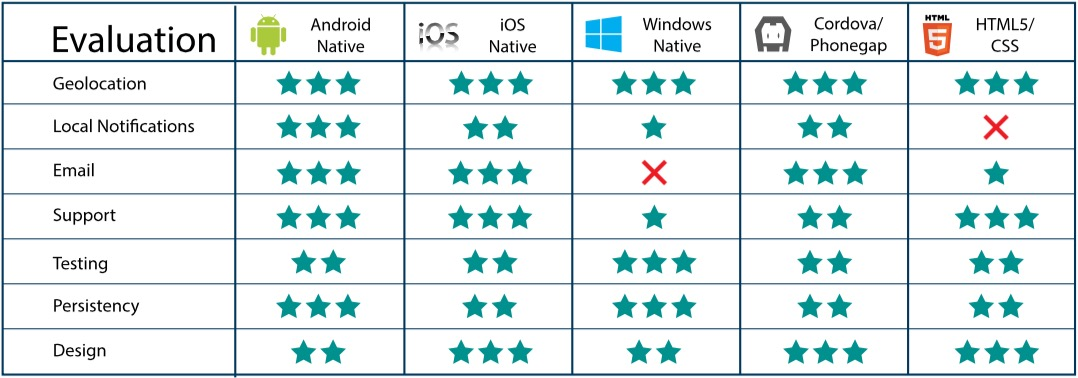
\includegraphics[scale=0.4]{resources/comparison.jpg}
\label{comparison}
\end{figure*}

Figure \ref{comparison} zeigt eine Gegenüberstellung der erreichten Punktzahlen der einzelnen Technologien. Während Android, iOS und Phonegap alle Probleme mit sehr hoher Punktzahl lösen könnten, gab es bei Windows und HTML5 des Öfteren schlechte Bewertungen und es gab sogar Features, die nicht umgesetzt werden konnten. Sowohl HTML5 bräuchte für lokale Notifications Backend-Unterstützung, als auch Windows beim Versenden von Emails mit Anhängen.

Bei der Nutzung von Geolocations und Ortungsdiensten haben alle Technologien die maximale Punktzahl erreicht, somit sind Anforderungen diesbezüglich für keine der Technologien ein K.O. Kriterium.

Im Bezug auf das Design haben die hybriden web-basierten Anwendungen die Nase vorn, wenn es um die Etablierung eines eigenen Designs geht. Sollen die Apps möglichst nativ aussehen, dann könnte es hier etwas aufwändiger werden und der Vorteil, dass bei Phonegap nur eine einzige App implementiert werden muss evtl. wegfallen. IOS ist vom Design her sehr schnell umsetzbar, sofern nur auf die Standard-Widgets zugegriffen wird. 


\section{Fazit}




%\bibliographystyle{abbrv}
%\bibliography{amos5}
\end{document}
